\subsection{Effect of GPS Coordinate Augmentation on Downstream Tasks}
\label{sec:downstream_gps_augmentation}

To evaluate whether explicit GPS coordinates improve LLM performance on geographic reasoning tasks, we augment two existing benchmarks with coordinate information and compare model accuracy before and after augmentation.

\paragraph{Datasets.}
We evaluate on two benchmarks:
\begin{itemize}[leftmargin=*, itemsep=2pt]
    \item \textbf{MapEval}~\cite{mapeval}: A benchmark of map-based questions covering trip planning, routing, nearby search, and POI queries. We augment the context by appending GPS reference coordinates for all mentioned locations. We filter to samples where all places were successfully geocoded (n=66).
    \item \textbf{Hierarchical Spatial}~\cite{fulman2024distortions}: A benchmark of 22 questions testing intercardinal direction judgments between cities, designed to expose spatial reasoning biases. We augment each city pair with their GPS coordinates.
\end{itemize}

\paragraph{Augmentation Method.}
For MapEval, we geocode all place names mentioned in the context and append a \texttt{[GPS Reference Coordinates]} section with latitude/longitude values (e.g., ``Cusco Cathedral: 13.5163°S, 71.9779°W''). For Hierarchical Spatial, we prepend each city's coordinates to the prompt (e.g., ``Portland, OR is located at coordinates (45.5202°N, 122.6742°W)'').

\begin{figure}[htbp]
\centering
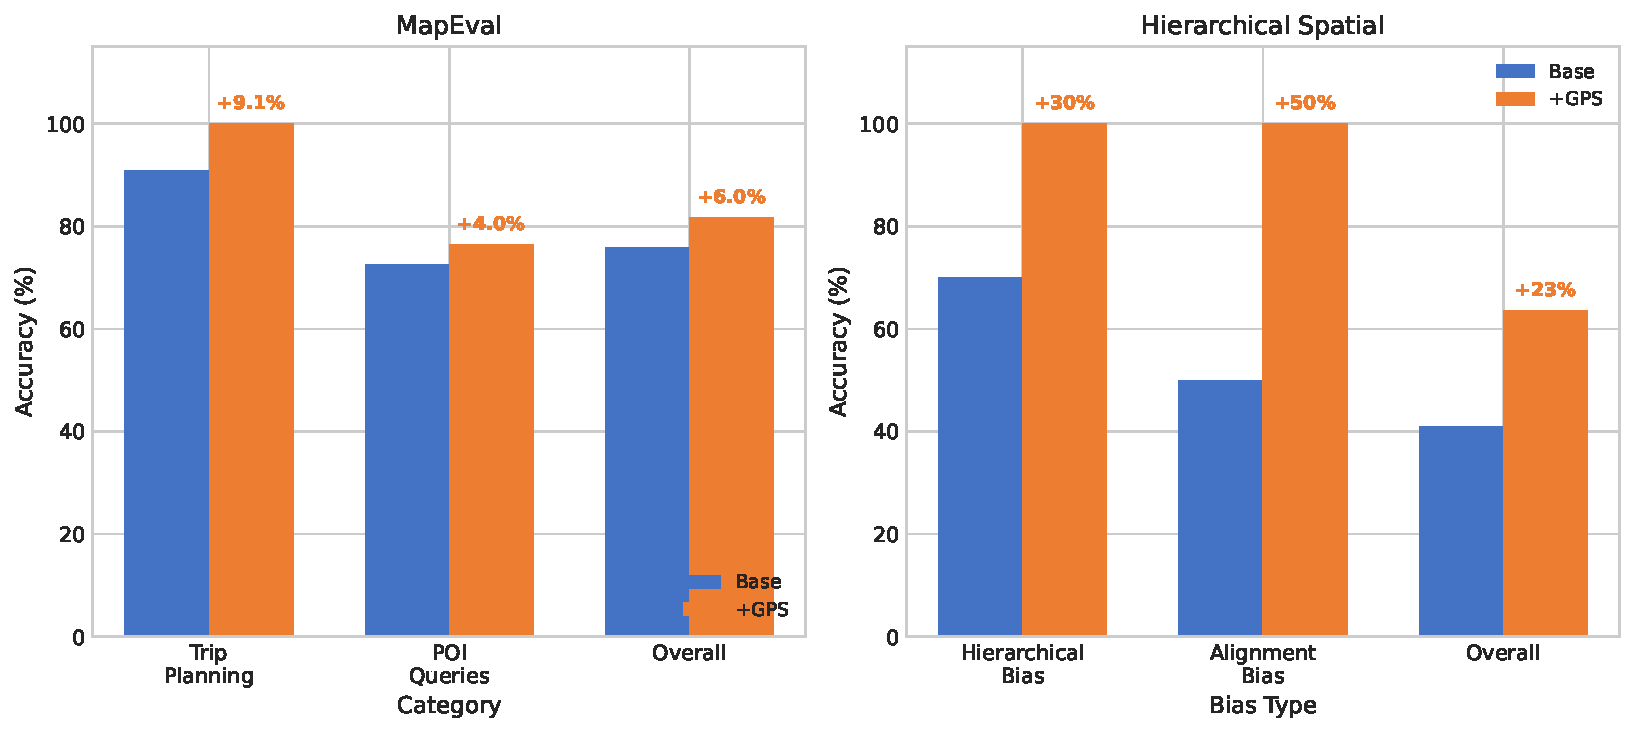
\includegraphics[width=\columnwidth]{figures/downstream_gps_augmentation.pdf}
\caption{Effect of GPS coordinate augmentation on downstream tasks. Left: MapEval shows modest improvement (+6.1\% overall) with 100\% geocoded samples. Right: Hierarchical Spatial shows substantial improvement (+22.7\%), with GPS coordinates eliminating hierarchical and alignment biases.}
\label{fig:downstream_gps}
\end{figure}

\begin{table}[htbp]
\centering
\caption{Effect of GPS coordinate augmentation on downstream task accuracy (\%). Results using GPT-4.1. MapEval filtered to 100\% geocoded samples.}
\label{tab:gps_augmentation_downstream}
\small
\begin{tabular}{llcccc}
\toprule
\textbf{Dataset} & \textbf{Category} & \textbf{N} & \textbf{Base} & \textbf{+GPS} & \textbf{$\Delta$} \\
\midrule
\multirow{4}{*}{\shortstack[l]{MapEval\\(100\% geocoded)}}
    & Trip planning & 11 & 90.9 & 100.0 & +9.1 \\
    & POI queries & 51 & 72.5 & 76.5 & +3.9 \\
    & Nearby search & 3 & 66.7 & 100.0 & +33.3 \\
    \cmidrule{2-6}
    & \textit{Overall} & \textit{66} & \textit{75.8} & \textit{81.8} & \textit{+6.1} \\
\midrule
\multirow{5}{*}{\shortstack[l]{Hierarchical\\Spatial}}
    & Hierarchical bias & 10 & 70.0 & 100.0 & +30.0 \\
    & Alignment bias & 4 & 50.0 & 100.0 & +50.0 \\
    & Proximity bias & 4 & 0.0 & 0.0 & 0.0 \\
    & Rotation bias & 4 & 0.0 & 0.0 & 0.0 \\
    \cmidrule{2-6}
    & \textit{Overall} & \textit{22} & \textit{40.9} & \textit{63.6} & \textit{+22.7} \\
\bottomrule
\end{tabular}
\end{table}

\paragraph{Findings.}
As shown in Figure~\ref{fig:downstream_gps} and Table~\ref{tab:gps_augmentation_downstream}, GPS augmentation produces consistent improvements when coordinate information is complete:

\begin{itemize}[leftmargin=*, itemsep=2pt]
    \item \textbf{MapEval}: On samples with 100\% geocoding coverage, accuracy improves by +6.1\% (75.8\%→81.8\%). Trip planning shows the largest gain (+9.1\%), reaching perfect accuracy, while POI queries improve by +3.9\%.

    \item \textbf{Hierarchical Spatial}: Substantial improvement (+22.7\%). GPS coordinates eliminate hierarchical bias (70\%→100\%) and alignment bias (50\%→100\%), where models previously made incorrect assumptions based on country-level geography (e.g., assuming Toronto is north of Portland because Canada is north of the US). However, proximity and rotation biases remain at 0\%, suggesting these errors stem from deeper spatial reasoning limitations rather than missing coordinate information.
\end{itemize}

These results demonstrate that GPS coordinates provide meaningful benefit (+6--23\%) when coordinate coverage is complete, particularly for tasks requiring precise spatial relationships or overcoming learned geographic biases.
